% -*- mode:flyspell; mode:latex  -*-

%%% Local Variables:
%%% TeX-master: "mu2e-36575"
%%% End:

%%%%%%%%%%%%%%%%%%%%%%%%%%%%%%%%%%%%%%%%%%%%%%%%%%%%%%%%%%%%%%%%%%%%%%%%%%%%% 
\section{Track Quality Selections}

%%%%%%%%%%%%%%%%%%%%%%%%%%%%%%%%%%%%%%%%%%%%%%%%%%%%%%%%%%%%%%%%%%%%%%%%%%%%%%
\subsection{\MuToEm\  Channel}
\label{sec:mumem_channel}

Selection of correctly reconstructed tracks plays a critical role in the search, and 
to improve rejection of poorly reconstructed  tracks, an MVA-based technique is used.
A MLP ANN is trained to distinguish between correctly reconstructed tracks
and mis-reconstructed ones, good tracks are selected by requiring the ANN score to be
above certain value.

In the Mu2e offline, two different track fits are used to determine the track parameters.
Both are using the same fitting algorithm, but the fits are performed with two different
hit ambiguity resolvers, a panel-based ambiguity resolver, or PAR, and a doublet-based
ambiguity resolver, or DAR. A track quality ANN has been trained only for one of them,
the PAR. 
%
We performed a similar training for the output of the DAR track fits.
%
Following \cite{MU2E_4595_ANN_TRAINING}, we used ROOT TMVA package to train a MLP ANN
with 8 input variables and one hidden layer. The following eight variables were used
as inputs:

\begin{itemize}
\item
  {\bf na } : number of ``active'' hits remaining on the track after the Kalman fit and used
  in the calculation of the fit $\chi^2$
\item
  {\bf nafract} : na/nhits , a ratio of the number of active hits to the total number
  of hits (after the seed fit)
\item
  ${\bf log_{10}{fcons}}$ : {\bf fcons}, or fit consistency is a probability-minded derivative
  from the track fit $\chi^2$. Logarithm of it is taken from the numerical considerations
\item
  {\bf momerr} : uncertainty on the reconstructed track momentum, returned by the fitter
\item
  {\bf t0err} : uncertainty on the reconstructed track time, T0, returned by the fitter
\item
  {\bf fda} : Nd/Na, fraction of ``doublet'' active hits
\item
  {\bf fza } : Nza/Na, fraction of activev hits with undefined drift direction
\item
  {\bf fma } : {\bf \red to be clarified}
\end{itemize}

The ANN training is aimed to optimize the separation of electron tracks reconstructed correctly, 
with $\Delta{P} = |P_{reco}-P_{true}| < 0.25$ MeV/c, or approximately within $2\sigma$ from the true
value, from tracks reconstructed with $\Delta{P} > 0.7$ MeV/c, or , approximately, $5\sigma$
above the true value.

Comparison between $P_{true}$ and $P_{reco}$ was performed in a plane corresponding to the
tracker front.
%
Used for the ANN training were tracks with |D0| < 100 mm and 0.5 < \tandip < 1. 

To choose between the PAR-based and DAR-based fitters, we compared performance of the
trained DAR ANN to the performance of the default for the offline v9\_0\_5 offline PAR ANN.
%
Using the CD3 choice of the signal region , 103.85 < P < 104.90 MeV/c, $T_0 > 700$ ns,
we compared performances of the two methods.
%
Figure \ref{fig:mumem_ann_operational_point_choice} shows the expected DIO background plotted
versus the CE reconstruction efficiency. Both are plotted in relative units, normalized
to the DIO background and CE efficiency of the PAR track selection with the default
cut on the ANN score $S_{PAR} > 0.8$ respectively.
%
Squares represent PAR track selection, circles - DAR track selection, red and black colors
correspond to the CE+1 batch mode pileup and CE+2 batch mode datasets correspondingly.
%
In all cases the background model comes from the DIO-weighted fele2s51b1 dataset -
electrons + 1 batch pileup. 

As follows from Figure \ref{fig:mumem_ann_operational_point_choice}, for the same expected 
background level, using the DAR tracks allows to increase acceptance by 4-5\%. One can also see,
that the choice of the PAR ANN operational point is quite close to the optimum - after the 
(1,1) point the PAR background starts increasing much faster than the PAR signal,
and the increase by 5\% comes along with the x2 higher DIO background.

For the DAR tracks, improving the signal acceptance by the same 5\% wrt the default offline
selection doesn't cost extra background. This determines the choices for SU2020 analyses: 

\begin{itemize}
\item
  SU2020 analyses use DAR tracks
\item
  the ANN operational point corresponds to the cut on the output of $S_{DAR} > 0.2$.
\end{itemize}

\begin{figure}[H]
\begin{tikzpicture}
  \node[anchor=south west,inner sep=0] at (0,0.) {
    % \node[shift={(0 cm,0.cm)},inner sep=0,rotate={90}] at (0,0) {}
    \makebox[\textwidth][c] {
      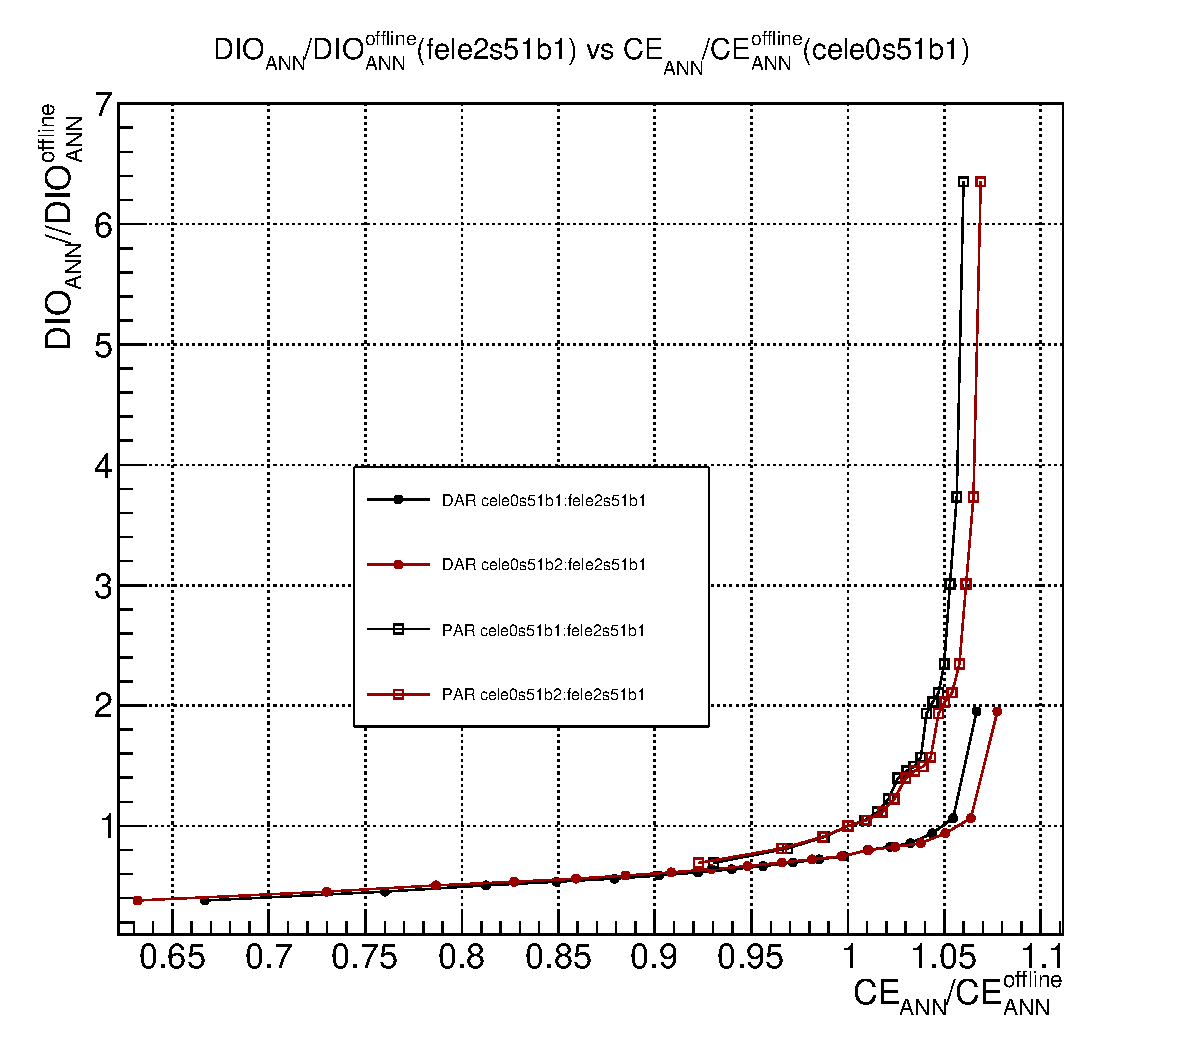
\includegraphics[width=0.8\textwidth]{figures/pdf/mumem_trq_ann_signal_vs_background}
    }
  };
  % \node [text width=6cm, scale=0.8] at (4.5,6.4) {mu2e-18894 by Kevin Lynch and Jim Popp};
\end{tikzpicture}
% \captionof{figure} {
\caption{
  \label{fig:mumem_ann_operational_point_choice}
  Choice of the ANN operational point. background numbers - from fele2s51b1,
  signal efficiency: black points: cele0s51b1; Red: cele0s51b2;
  Compared to PAR track selection $S_{PAR} > 0.8$, selecting DAR tracks with $S_{DAR} > 0.2$ 
  improves acceptance in the CD3 signal region of [103.85,104.90] by 4-5\%, 
  while keeping the DIO background at a lower level.
  {\color{red} {\bf *** update caption **}}
}
\end{figure}

Figure \ref{fig:mumem_dar_vs_par_ann} compares the track momentum resolution distributions 
for DAR and PAR tracks reconstructed in {\bf cele0s61b2} dataset and selected with different
cuts on the corresponding ANN score.

In Figure \ref{fig:mumem_dar_vs_par_ann}(a) the operational points for DAR and PAR track selection
are chosen to give the same expected background, in Figure \ref{fig:mumem_dar_vs_par_ann}(b) -
the same track selection efficiency. Higher high-momentum tail in the distribution for PAR
tracks is clearly visible.

\begin{figure}
\hspace{-0.6in}
\begin{tikzpicture}
  \node[anchor=south west,inner sep=0] at (0,0.) {
    % \node[shift={(0 cm,0.cm)},inner sep=0,rotate={90}] at (0,0) {}
    % \makebox[\textwidth][c] {
    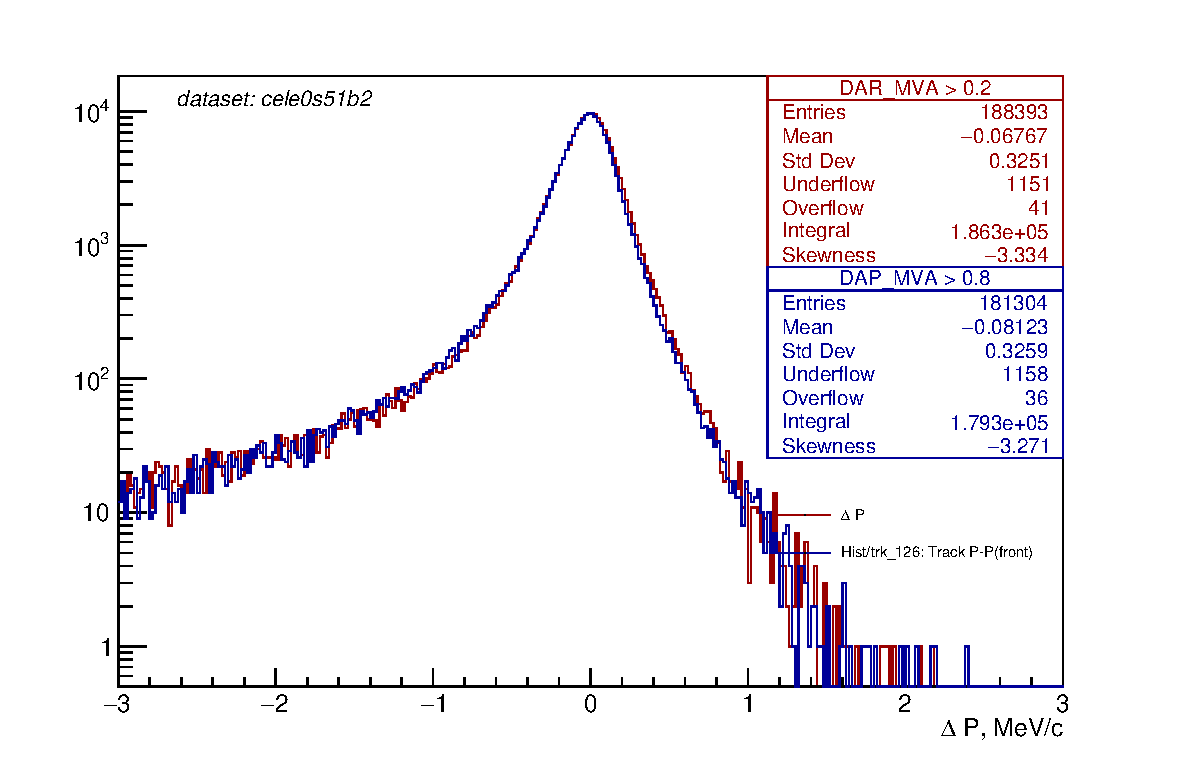
\includegraphics[width=0.64\textwidth]{figures/pdf/figure_00114_cele0s51b2_track_comp_ffff_1070_trk_214_vs_126_dpf}
    % }
  };
  \node [text width=1cm, scale=0.8] at (3.,4.5) {(a)};
  \node[anchor=south west,inner sep=0] at (10.5,0.) {
    % \node[shift={(0 cm,0.cm)},inner sep=0,rotate={90}] at (0,0) {}
    % \makebox[\textwidth][c] {
    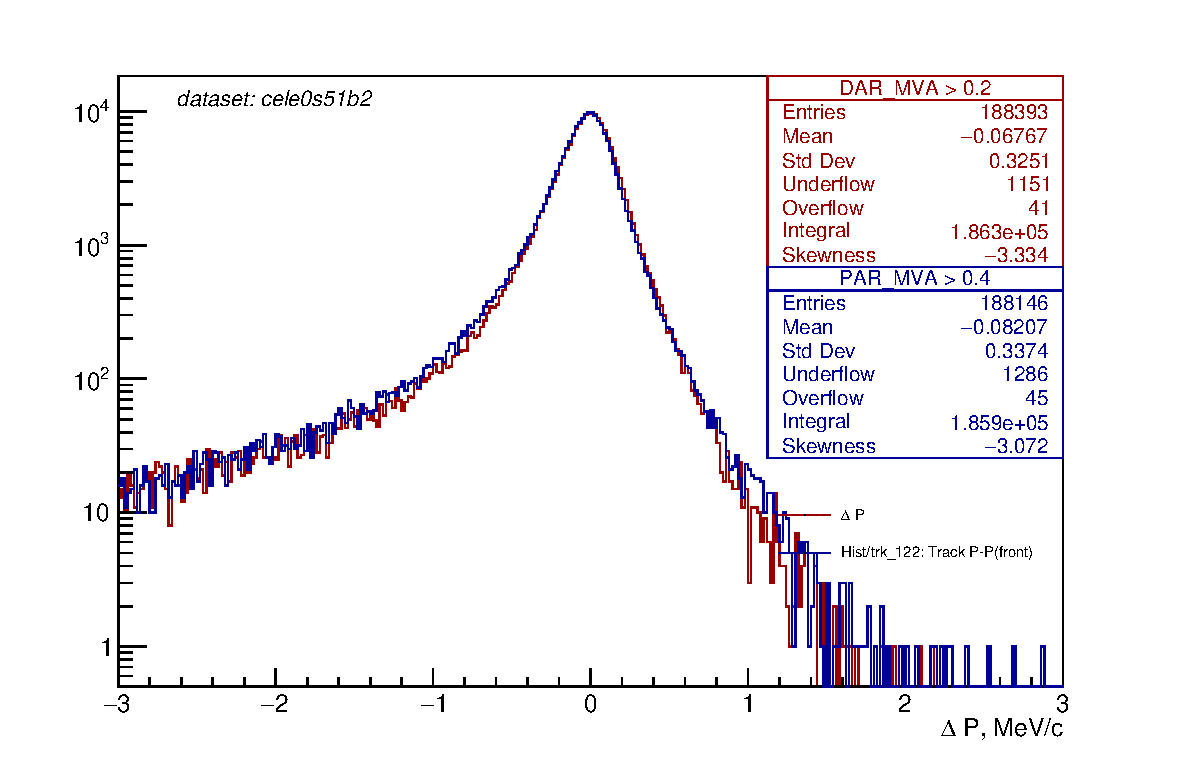
\includegraphics[width=0.64\textwidth]{figures/pdf/figure_00116_cele0s51b2_track_comp_ffff_1070_trk_214_vs_122_dpf}
    % }
  };
  \node [text width=1cm, scale=0.8] at (13.5,4.5) {(b)};
\end{tikzpicture}
% \captionof{figure} {
\caption{
  \label{fig:mumem_dar_vs_par_ann}
  DAR vs PAR track selection efficiency for two operational points: 
  (a): DAR and PAR selections correspond to the same background, (b): DAR and PAR selections correspond
  to the same efficiency. \\
  The right-side tail, determined by the misreconstructed tracks, is a measure of the track selection quality 
}
\end{figure}

Improvements in the track reconstruction, for the same selection efficiency, result in a significantly better
rejection of the misreconstructed tracks. Figure \ref{fig:dio_delta_p_1036_1050} shows the $\Delta{P}$ distribution
for the simulated DIO electrons (DIO-weighted fele2s51b1) with the reconstructed track momenta
in [103.6, 105.0] MeV/c. From that distribution one can easily quantify importance of the relative contribution
of tracks with $\Delta{P}$ above certain threshold.  In particular, tracks with significantly mis-reconstructed
momenta, $\Delta{P} > 0.5$ MeV, represent about 0.23 of the expected DIO background, about 50\% lower than 0.355,
estimated for the same momentum window in \cite{MU2E_4595_ANN_TRAINING}..

\begin{figure}
  \begin{tikzpicture}
    \node[anchor=south west,inner sep=0] at (0,0.) {
      % \node[shift={(0 cm,0.cm)},inner sep=0,rotate={90}] at (0,0) {}
      \makebox[\textwidth][c] {
        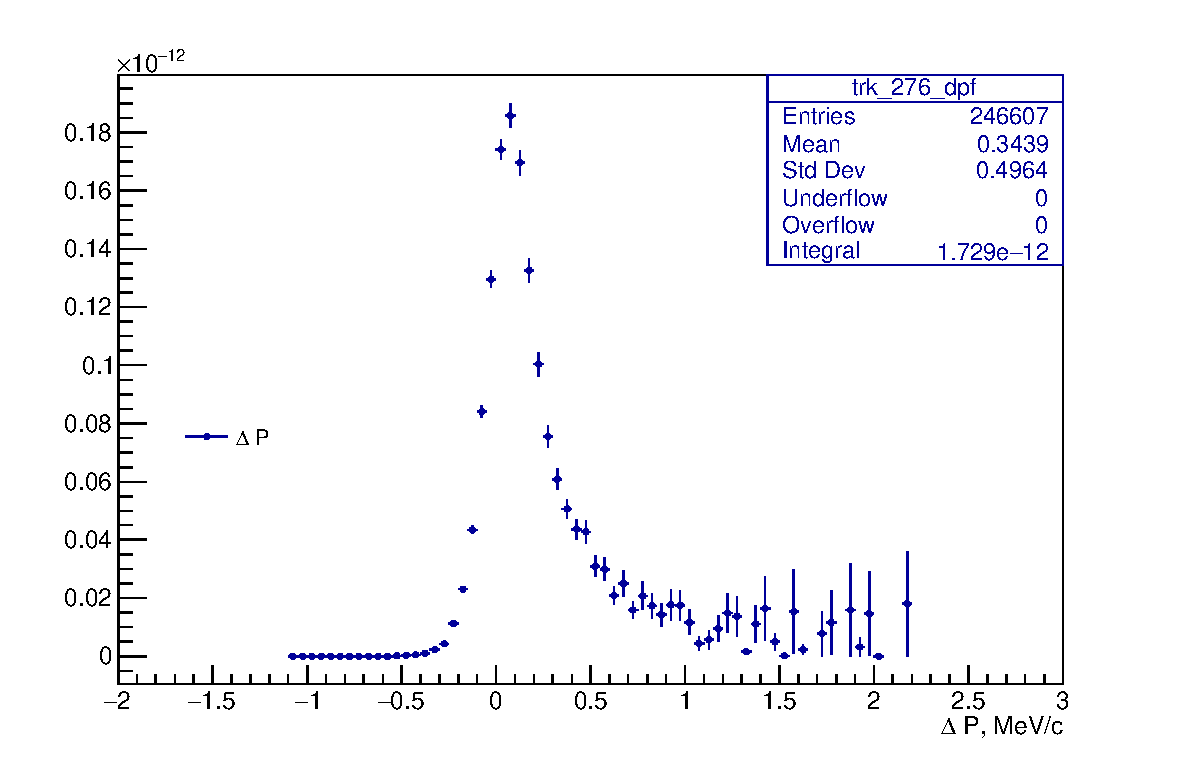
\includegraphics[width=0.99\textwidth]{figures/pdf/figure_00111_fele2s51b1_track_comp_ffff_1070_trk_276_dpf}
      }
    };
    % \node [text width=6cm, scale=0.8] at (4.5,6.4) {mu2e-18894 by Kevin Lynch and Jim Popp};
  \end{tikzpicture}
  % \captionof{figure} {
  \caption{
    \label{fig:dio_delta_p_1036_1050} 
    $\Delta P ~=~ P_{reco} -P_{true}$ distribution for simulated DIO background in the region [103.6,105.0] MeV.
    77.2\% of reconstructed events in this region are expected to have $\Delta P < 0.5$ MeV/c
  }
\end{figure}

As a cross-check, we used the TMVA package to train a BDT-based track quality classifier.
Similar to \cite{MU2E_33150_ANN_TRAINING}, we found that the MLP ANN performed slightly better,
so current analysis uses a MLP ANN-based track quality selection.

To explore the parameter space, the definition of a ``mis-reconstructed track'' has been varied and
a similar ANN has been trained to discriminate tracks reconstructed with $\Delta{P} < 0.25$ MeV/c
from tracks with $\Delta{P} > 0.6$ MeV/c. No improvement in the DIO
suppression in the region [103.85, 104.9] MeV/c was observed. 

%%%%%%%%%%%%%%%%%%%%%%%%%%%%%%%%%%%%%%%%%%%%%%%%%%%%%%%%%%%%%%%%%%%%%%%%%%%%%%
\newpage
\subsection{\MuToEp\ Channel}
\label{sec:mumep_channel}

To select tracks in \MuToEp\ channel, a e+ + 1-batch mode pileup ({\bf cpos0s51b1}) dataset 
has been used to train a MLP ANN to discriminate between correctly and mis-reconstructed positron tracks.
The ANN configuration and the definitions of a well reconstructed and mis-reconstructed tracks are
the same as described in Section \ref{sec:mumem_channel}.

Figure \ref{fig:mumep_trq_ann} compares the expected background vs the signal efficiency curves,
in relative scale, for PAR (squares) and DAR(circles) tracks.
As in Figure \ref{fig:mumem_ann_operational_point_choice}, the expected background and the signal
efficiency are plotted relative to the background and signal efficiency expected for the default
positive track selection implemented in offline v9\_0\_5.
The background definition, however, is different. Unlike in \MuToEm\ channel, in \MuToEp\ there is
no well defined background process which contribution could be used as a measure of mis-reconstruction.
The RMC contribution depends on the assumptions about the RMC photon momentum distribution and,
in particular, its endpoint. Because of this, the background in Figure \ref{fig:mumem_ann_operational_point_choice}
is defined as the expected number of events with the misreconstructed momentum $\Delta{P} > 1.0$ MeV.
The signal is integrated over the [90.5,92.5] MeV/c momentum window,

Figure \ref{fig:mumem_ann_operational_point_choice}.(b) shows the same performance curves
as \ref{fig:mumem_ann_operational_point_choice}.(a), but with the vertical axis in logarithmic scale.
It is interesting to see, that for given background definition, the background increases exponentially
with the signal acceptance for both types of tracks.

For the same signal acceptance, the ANN-based selection of DAR tracks results in lower
background, so the sensitivity estimate in \MuToEp\ channel also uses the DAR tracks. 

At to the choice of the operational point, cut $S_{DAR} > 0.2$ improves the signal acceptance
by 10\%, while increasing the background by 15\%. Relaxing the cut and moving the cut value
to $S_{DAR} > 0.15$ adds another 2\% to the CP acceptance, while the background grows much faster
and becomes $B_{DAR}/B_{PAR}^{default} = 1.5,$
Thus, the default cut on the $S_{DAR}^-$ is the same as in the electron channel:  $S_{DAR}^- > 0.2$

An attempt to train a similar ANN for PAR tracks, somewhat surprisingly, didn't improve the performance
of the ANN-based PAR track selection, leaving a potential for further improvements.

\begin{figure}[H]
  \hspace{-0.6in}
  \begin{tikzpicture}
    \node[anchor=south west,inner sep=0] at (0,0.) {
      % \node[shift={(0 cm,0.cm)},inner sep=0,rotate={90}] at (0,0) {}
      % \makebox[\textwidth][c] {
      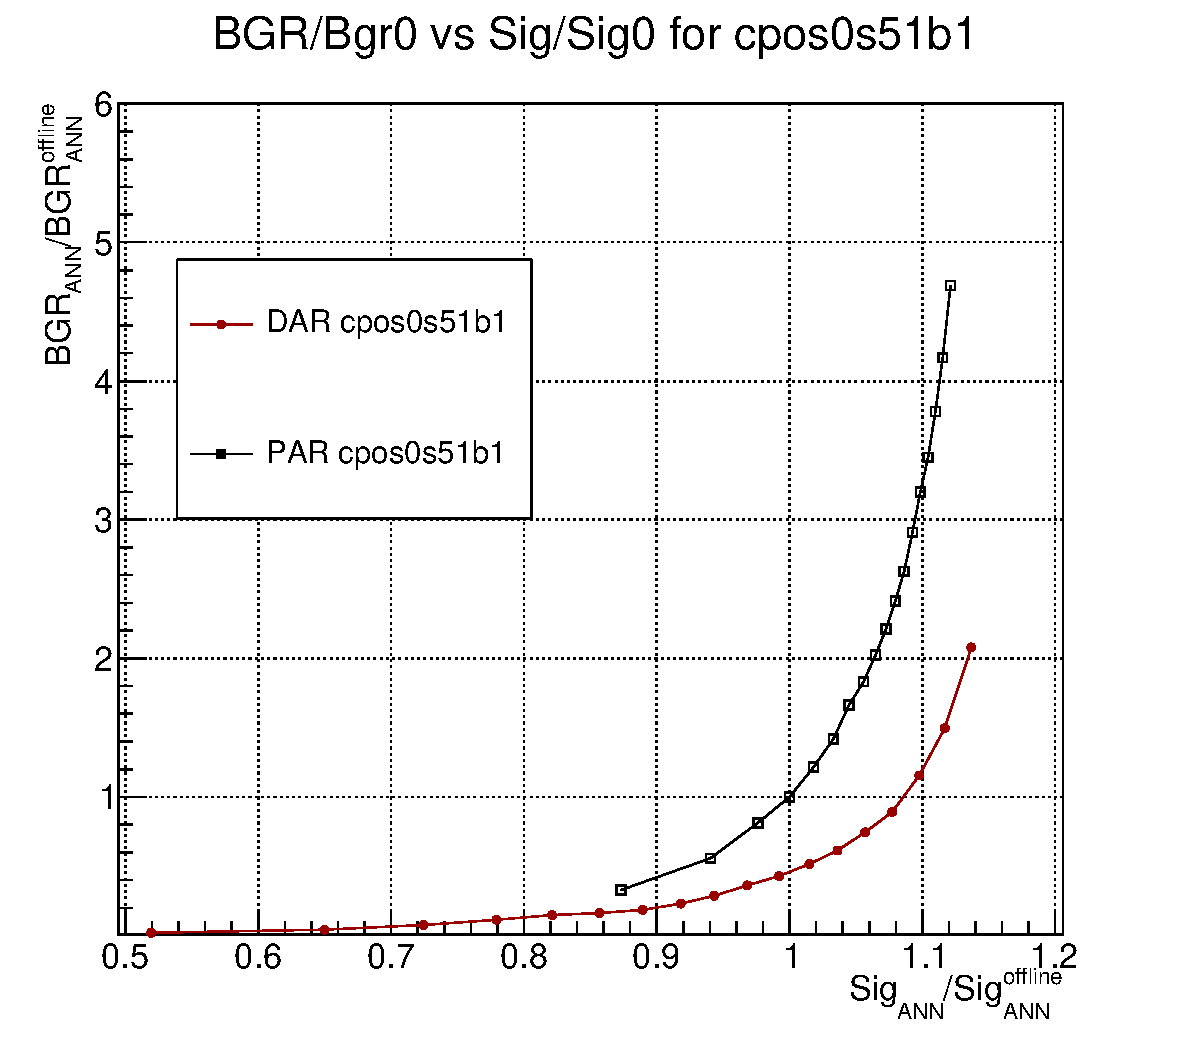
\includegraphics[width=0.55\textwidth]{figures/pdf/mumep_trq_ann_signal_vs_background_lin}
      % }
    };
    \node [text width=1cm, scale=1.0] at (3.,3.5) {(a)};
    \node[anchor=south west,inner sep=0] at (10,0.) {
      % \node[shift={(0 cm,0.cm)},inner sep=0,rotate={90}] at (0,0) {}
      % \makebox[\textwidth][c] {
      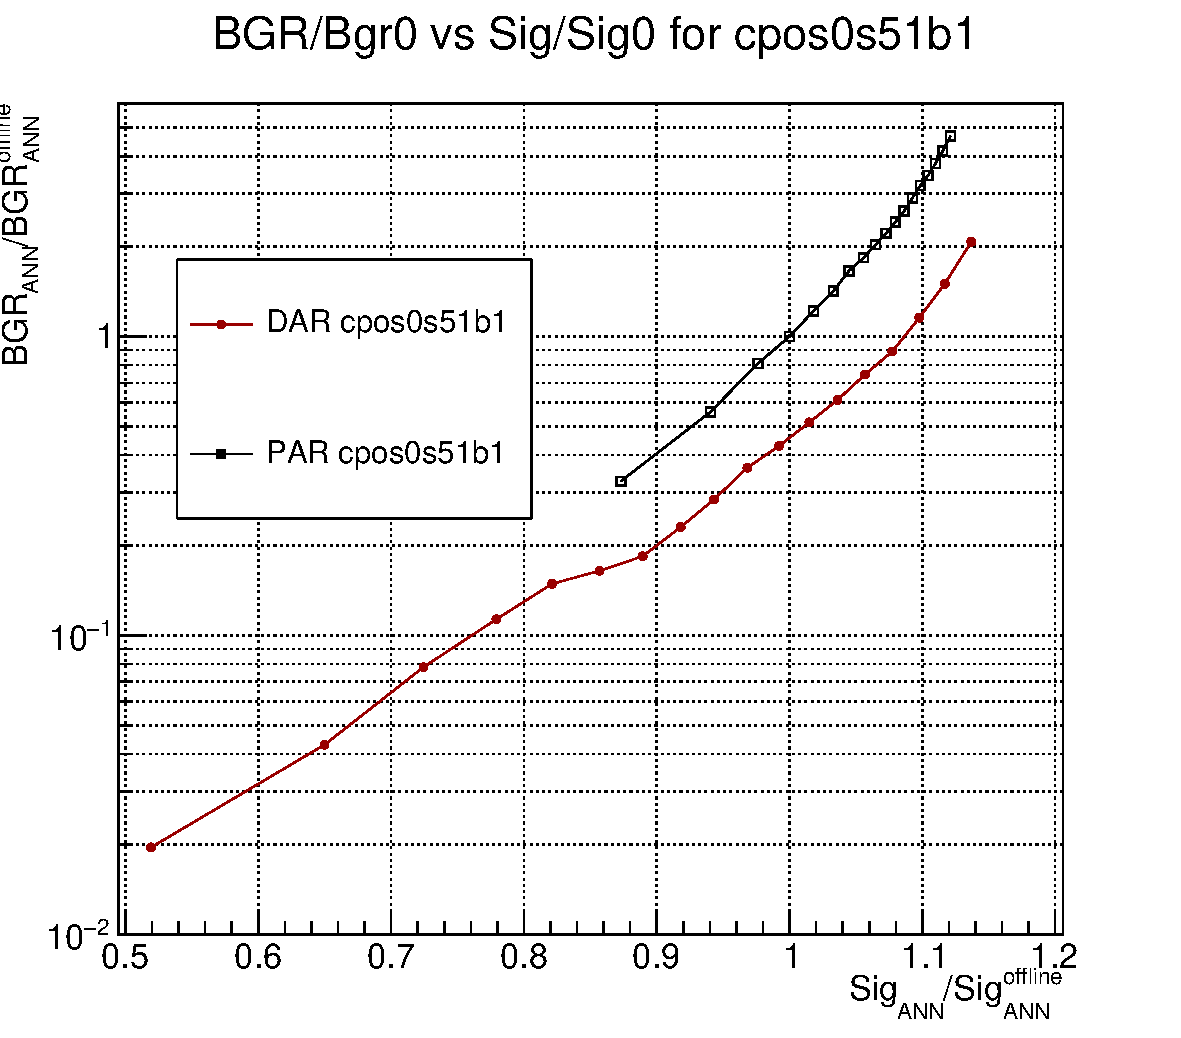
\includegraphics[width=0.55\textwidth]{figures/pdf/mumep_trq_ann_signal_vs_background_log}
      % }
    };
    \node [text width=1cm, scale=1.0] at (13.,3.5) {(b)};
  \end{tikzpicture}
  % \captionof{figure} {
  \caption{
    \label{fig:mumep_trq_ann} 
    DAR (Circles) vs PAR (squares) background vs track selection efficiency.
    Signal: {\bf cpos0s51b1} , signal window, background:{\bf cpos0s51b1} , tracks with $\Delta{P} > 1.0$ MeV.
    Both signal and background are measured in units of signal and background corresponding to the selection
    using default Offline v9\_0\_5 ANN-based track selection, $S_{PAR}^+ > 0.8$.
  }
\end{figure}

%%%%%%%%%%%%%%%%%%%%%%%%%%%%%%%%%%%%%%%%%%%%%%%%%%%%%%%%%%%%%%%%%%%%%%%%%%%%%%
\subsection{Testing charge symmetry of the ANN-based track selection}

It is worth noting that the track parameters used for ANN training don't depend explicitly
on the reconstructed track sign. One could therefore expect the efficiency of the ANN-based
track selection to be charge-symmetric. To check this hypothesis, Figure \ref{fig:su2020_mva_test_dar}
compares efficiency of the ANN-based selection for 105 MeV electrons and 105 MeV positrons, where
in both cases the tracks were selected with the ANN trained on negative tracks.

Figure \ref{fig:su2020_mva_test_dar} confirms that for the same track momentum, the ANN-based  selection
is charge-symmetric with an accuracy better than 0.5\%.

The third, and the only visible in Figure \ref{fig:su2020_mva_test_dar} distribution corresponds to
selection of 105 MeV electron tracks using ANN trained on  92 MeV positrons as described in
Section \ref{sec:mumep_channel}. One can expect efficiency of this selection to be sub-optimal,
rather surprisingly, efficiency is reduced by less than 4\%.

Observed charge symmetry allows to use one common ANN to select tracks in all channels in \MuToEm\ search 
and another one - for track selection in all channels in \MuToEp\ analysis.

\begin{figure}
  % \hspace{-0.6in}
  \begin{tikzpicture}
    \node[anchor=south west,inner sep=0] at (0,0.) {
      % \node[shift={(0 cm,0.cm)},inner sep=0,rotate={90}] at (0,0) {}
      \makebox[\textwidth][c] {
        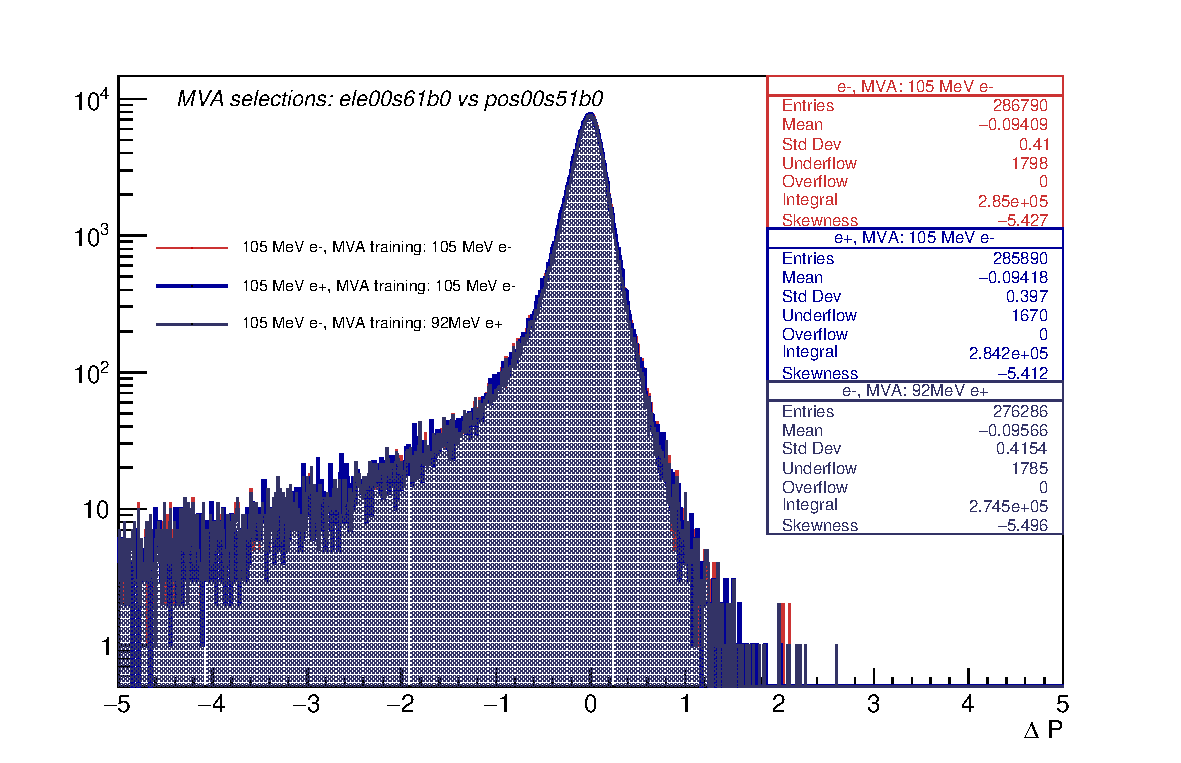
\includegraphics[width=0.95\textwidth]{figures/pdf/figure_00231_su2020_mva_test_dar}
      }
    };
    % \node [text width=6cm, scale=0.8] at (4.5,6.4) {mu2e-18894 by Kevin Lynch and Jim Popp};
  \end{tikzpicture}
  % \captionof{figure} {
  \caption{
    \label{fig:su2020_mva_test_dar} 
    Electron and positron selection, 105 MeV , positron selection - 90 MeV/c
  }
\end{figure}


%%%%%%%%%%%%%%%%%%%%%%%%%%%%%%%%%%%%%%%%%%%%%%%%%%%%%%%%%%%%%%%%%%%%%%%%%%%%%%
\subsection{Final track quality selections}

The finalized track selection includes three cuts. The track impact parameter cut selects tracks consistent 
with coming from the stopping target, the track $\tan\lambda$ cut, in essense, is an anti-cosmics cut, and 
its final value needs to be optimized. The cut on the ANN output, or score, variable selects
well reconstucted tracks.

\begin{table}[h!]
  \begin{center}
    \begin{tabular}{l|c|c} % <-- Changed to S here.
      \textbf{Cut variable} & \textbf{Cut value} & \textbf{``N-1'' Efficiency for CE}\\
      \hline
      track impact parameter,  D0 & | D0 | < 100 mm           &   0.990    \\
      track dip angle, \tandip    & $ 0.5< \tan \lambda < 1.$ &   0.909    \\
      track quality ANN score, $S_{TRQ}$      & $S_{TRQ} > 0.2$            &   0.901    \\
    \end{tabular}
  \end{center}
  \caption{
    \label{tab:trq_cuts}
    Final Track quality selection
  }
\end{table}

Table \ref{table:ce_trq_efficiency_vs_pileup} benchmarks the selection efficiencies for fits using two different
anbiguity resolvers

\begin{table}[h!]
  \begin{center}
    \caption{Efficiency for different levels of pile-up occupancy}
    \label{tab:table1}
    \begin{tabular}{l|c|c|c} % <-- Changed to S here.
      \textbf{pileup}    & Eff DAR &  Efficiency PAR  &  DAR/PAR   \\
      \hline                                                           
      CE                 &  0.152  &   0.149          &  1.02      \\
      CE+1-batch pileup  &  0.152  &   0.146          &  1.04      \\
      CE+2-batch pileup  &  0.149  &   0.143          &  1.04      \\
    \end{tabular}
  \end{center}
  \caption{
    \label{table:ce_trq_efficiency_vs_pileup_1} 
    conversion electron (CE) track selection efficiency for different levels of pileup and momentum window [103,105.0]  
    and T0 > 700 ns
  }
\end{table}


% PAR 1b:107810

\begin{table}[h!]
  \label{table:ce_trq_efficiency_vs_pileup_2} 
  \begin{center}
    \begin{tabular}{l|c|c|c} % <
      \textbf{pileup}    & Eff DAR &  Efficiency PAR  &  DAR/PAR   \\
      \hline                                                           
      CE                 &  0.111  &   0.104          &  1.07      \\
      CE+1-batch pileup  &  0.113  &   0.108          &  1.05      \\
      CE+2-batch pileup  &  0.111  &   0.105          &  1.05      \\
    \end{tabular}
  \end{center}
  \caption{
    conversion electron (CE) track selection efficiency for different levels of pileup and momentum window [103.85,105.0] 
    and T0 > 700 ns
  }
\end{table}





